\section{Calcul des coefficients de la CI3 par moindres carrés sur l'impédance}

    On se donne \(N_x\) \(k_x\) et \(N_y\) \(k_y\). Il existe donc \(N_k=N_xN_y\) couples tels que \((k_{xi},k_{yj}) = (k_x,k_y)_{(j-1)N_x+i}\).
    \begin{defn}
      Soit \(\ps{\cdot}{\cdot}\) le produit scalaire usuel de \(\CC^{N_{k}}\) et \(\norm{\cdot}\) la norme associée.
      \begin{equation*}
        \ps{a}{b} = \sum_{i=1}^{N_k} \conj{a_i} b_i
      \end{equation*}
      Soit \(\ps{\cdot}{\cdot}_F\) le produit scalaire usuel de \(\mathcal{M}_2(\CC)\) et \(\norm{\cdot}_F\) la norme associée.
      \begin{equation*}
        \ps{\mA}{\mB}_F = \operatorname{Tr}(\conj{\mA^t}\mB)
      \end{equation*}
    \end{defn}

  \subsection[Expression de la fonctionnelle JZ]{Expression de la fonctionnelle \(J_Z\)}

    \begin{defn}
      On définit \(\mH_{CI3}\) la fonction de \(\RR \times \RR \times \mathcal{M}_2(\CC) \rightarrow \mathcal{M}_{4\times5}(\CC)\) telle que
      \begin{equation*}
        \mH_{CI3}(k_x,k_y,\mZ) = \begin{bmatrix}
        1 & \hat{\mLD}(k_x,k_y)_{11} & -\hat{\mLR}(k_x,k_y)_{11} & -\left(\hat{\mLD}(k_x,k_y)\mZ\right)_{11} & \left(\hat{\mLR}(k_x,k_y)\mZ\right)_{11}
        \\
        0 & \hat{\mLD}(k_x,k_y)_{12} & -\hat{\mLR}(k_x,k_y)_{12} & -\left(\hat{\mLD}(k_x,k_y)\mZ\right)_{12} & \left(\hat{\mLR}(k_x,k_y)\mZ\right)_{12}
        \\
        0 & \hat{\mLD}(k_x,k_y)_{21} & -\hat{\mLR}(k_x,k_y)_{21} & -\left(\hat{\mLD}(k_x,k_y)\mZ\right)_{21} & \left(\hat{\mLR}(k_x,k_y)\mZ\right)_{21}
        \\
        1 & \hat{\mLD}(k_x,k_y)_{22} & -\hat{\mLR}(k_x,k_y)_{22} & -\left(\hat{\mLD}(k_x,k_y)\mZ\right)_{22} & \left(\hat{\mLR}(k_x,k_y)\mZ\right)_{22}
        \end{bmatrix}
      \end{equation*}
      On définit \(b\) la fonction de \(\mathcal{M}_2(\CC) \rightarrow \mathcal{M}_{4\times1}(\CC)\) telle que
      \begin{equation*}
        b(\mZ) = \begin{bmatrix}
        \mZ_{11}
        \\
        \mZ_{12}
        \\
        \mZ_{21}
        \\
        \mZ_{22}
        \end{bmatrix}
      \end{equation*}
    \end{defn}

    \begin{prop}
      Soit \(X = (a_0,a_1,a_2,b_1,b_2)\), \((k_x,k_y)\) fixé et \(\hat\mZ_{ex}\) l'opérateur d'impédance exact du plan, alors
      \begin{equation*}
        \argmin{X\in\CC^5} \norm{\hat\mZ_{CI3}(k_x,k_y,X) - \hat\mZ_{ex}(k_x,k_y)} = \argmin{X\in\CC^5} \norm{\mH_{CI3}(k_x,k_y,\hat\mZ_{ex}(k_x,k_y))X - b(\hat\mZ_{ex}(k_x,k_y))}
      \end{equation*}
    \end{prop}

    \begin{proof}
      On rappelle que dans la section précédente, on a introduit
      \begin{multline*}
        \hat{\mZ}_{CI3}(k_x,k_y) = \left(\mI + b_1 \hat{\mLD}(k_x,k_y) - b_2 \hat{\mLR}(k_x,k_y) \right)^{-1}\\\left(a_0 \mI + a_1 {\hat{\mLD}(k_x,k_y)} - a_2 {\hat{\mLR}(k_x,k_y)}\right)
      \end{multline*}
      On pose
      \begin{align*}
        \hat\mZ_D(k_x,k_y) &= \mI + b_1 \hat{\mLD}(k_x,k_y) - b_2 \hat{\mLR}(k_x,k_y)
        \\
        \hat\mZ_N(k_x,k_y) &= a_0 \mI + a_1 {\hat{\mLD}(k_x,k_y)} - a_2 {\hat{\mLR}(k_x,k_y)}
      \end{align*}

      \begin{align*}
      &{}~ \argmin{X\in\CC^5} \norm{\hat\mZ_{CI3}(k_x,k_y,X) - \hat\mZ_{ex}(k_x,k_y)}
      \\
      & = \argmin{X\in\CC^5} \norm{\hat\mZ_D(k_x,k_y)^{-1}\hat\mZ_N(k_x,k_y) - \hat\mZ_{ex}(k_x,k_y) }
      \\
      &= \argmin{X\in\CC^5} \norm{\hat\mZ_D(k_x,k_y)^{-1}\left(\hat\mZ_N(k_x,k_y) - \hat\mZ_D(k_x,k_y)\hat\mZ_{ex}(k_x,k_y)\right) }
      \\
      &= \argmin{X\in\CC^5} \norm{\hat\mZ_N(k_x,k_y) - \hat\mZ_D(k_x,k_y)\hat\mZ_{ex}(k_x,k_y)}
      \\
      &= \argmin{X\in\CC^5} \norm{\hat\mZ_N(k_x,k_y) - \left(b_1 \hat{\mLD}(k_x,k_y) - b_2 \hat{\mLR}(k_x,k_y)\right)\hat\mZ_{ex}(k_x,k_y) - \hat\mZ_{ex}(k_x,k_y) }
      \\
      &= \argmin{X\in\CC^5} \norm{\mH_{CI3}(k_x,k_y,\hat\mZ_{ex}(k_x,k_y))X - b(\hat\mZ_{ex}(k_x,k_y))}
      \end{align*}
    \end{proof}

    \begin{defn}
      On définit \(\mA_{CI3}\) la matrice de \(\mathcal{M}_{4N_xN_y\times5}(\CC)\) telle que
      \begin{equation*}
        \mA_{CI3} = 
        \begin{bmatrix}
          \mH_{CI3}(k_{x1},k_{y1},\hat\mZ_{ex}(k_{x1},k_{y1}))
          \\
          \vdots
          \\
          \mH_{CI3}(k_{xi},k_{yj},\hat\mZ_{ex}(k_{xi},k_{yj}))
          \\
          \vdots
          \\
          \mH_{CI3}(k_{xN_x},k_{yN_y},\hat\mZ_{ex}(k_{xN_x},k_{yN_y}))
        \end{bmatrix}
      \end{equation*}
      On définit \(g\) la matrice de \(\mathcal{M}_{4N_xN_y\times1}(\CC)\) telle que
      \begin{equation*}
        g = 
        \begin{bmatrix}
          b(\hat\mZ_{ex}(k_{x1},k_{y1}))
          \\
          \vdots
          \\
          b(\hat\mZ_{ex}(k_{xi},k_{yj}))
          \\
          \vdots
          \\
          b(\hat\mZ_{ex}(k_{xN_x},k_{yN_y}))
        \end{bmatrix}
      \end{equation*}
    \end{defn}

    On peut alors calculer les coefficients de la CI3
    \begin{defn}
      On définit la fonctionnelle \(J_Z\)
      \begin{equation*}
        J_Z(X) = \norm{{\mA}_{CI3}X - {g}}^2
      \end{equation*}
    \end{defn}

    \begin{thm}[Minimisation sans contraintes pour la CI3]
      Les coefficients de la CIOE sont solutions du problème

      Trouver \(X^* \in \CC^5\) tel que
      \begin{equation*}
        X^* = \argmin{X\in \CC^5}  J_Z(X)
      \end{equation*}
    \end{thm}

    \begin{prop}
      \label{prop:plan:minimisation:minimum_sans_contraintes}
      Si \(\conj{\mA_{CI3}^t}\mA_{CI3}\) est inversible alors
      \begin{equation*}
        X^* = (\conj{\mA_{CI3}^t}\mA_{CI3})^{-1}(\conj{\mA_{CI3}^t}g)
      \end{equation*}
    \end{prop}

    \begin{proof}
      \begin{align*}
      J_Z(X) &= \norm{\mA_{CI3}X - g}^2
      \\
      &= \ps{\mA_{CI3}X - g}{\mA_{CI3}X - g}
      \intertext{le produit scalaire est hermitien donc}
      &=\ps{\mA_{CI3}X}{\mA_{CI3}X} - \ps{\mA_{CI3}X}{g} - \ps{g}{\mA_{CI3}X} + \ps{g}{g}
      \\
      &=\ps{X}{\conj{\mA_{CI3}^t}\mA_{CI3}X} - \ps{X}{\conj{\mA_{CI3}^t}g} - \ps{\conj{\mA_{CI3}^t}g}{X} + \ps{g}{g}
      \end{align*}
      Si la matrice \(\conj{\mA_{CI3}^t}\mA_{CI3}\) est inversible, comme elle est par définition hermitienne et positive alors la fonctionnelle est quadratique. Donc il existe un unique minimum où le gradient de cette fonctionnelle s'annule. Or
      \begin{align*}
        \nabla J_Z(X^*) &= 2\conj{\mA_{CI3}^t}\mA_{CI3}X^* - 2\conj{\mA_{CI3}^t}g
        \\ 
        &= 0
      \end{align*}
    \end{proof}

    Nous n'avons pas réussi à démontrer que cette matrice, associée à la CIOE CI3, était définie pour tout empilement et toute incidence.

    \begin{thm}[Minimisation avec contraintes pour la CI3]

      Soit \(\CSU[3]{CI3}\) le sous-espace de \(\CC^5\) issu de la définition \ref{def:csu:ci3-3}.
      Alors les coefficients de la CIOE respectant cette CSU sont solutions du problème

      Trouver \(X^* \in \CC^5\) tel que
      \begin{equation*}
        X^* = \argmin{X\in \CSU[3]{CI3}}  J_Z(X)
      \end{equation*}
    \end{thm}

  \subsection{Existence et unicité du minimum pour d'autres CIOE}

    \begin{prop}
      Il existe un unique minimum si la matrice \(\mM=\conj{\mH^t}{\mH}\) est inversible
    \end{prop}

    \begin{proof}
      On remarque que la fonctionnelle \(F\) est quadratique si la matrice \(\conj{\mH^t}{\mH}\) est hermitienne définie positive. Une matrice \(\mA\) est hermitienne si \(\forall x, \conj{x^t}\mA x \in \RR\), elle est hermitienne positive si \(\forall x, \conj{x^t}\mA x \in \RR^+\) et elle est hermitienne définie positive si \(\forall x\not=0, \conj{x^t}\mA x \in \RR^{+*}\).

      On remarque que par construction, notre matrice \(\mM\) est hermitienne positive. Il reste à montrer qu'elle est définie.
    \end{proof}

    \begin{prop}
      S'il existe un unique minimum \(X_{CI}^*\), celui-ci vaut
      \[
        X_{CI}^* = \left(\conj{\mH_{CI}^t}{\mH_{CI}}\right)^{-1}\conj{\mH_{CI}^t}b
      \]
    \end{prop}

    \begin{proof}
      C'est une application directe de \(\tgrad{} F(CI) = 0 \), avec la propriété précédente.
    \end{proof}

    \subsubsection{Existence du minimum pour la CI01}

      \begin{prop}
        La matrice \({\mM}_{CI01}\) associée à la CI01 est inversible, donc définie, si et seulement s'il existe au moins 2 couples \((k_{x},k_{y})\) différents.
      \end{prop}

      \begin{proof}
        Soit \(t\) le vecteur de \(\RR^{N_{k}}\) tel que \(t_{(j-1)N_x+i} = k_{xi}^2 + k_{yj}^2\) et \(1\) le vecteur de \(\RR^{N_{k}}\) où tous ces éléments valent \(1\). On a l'expression suivante de \({\mM}\)

        \begin{equation*}
          {\mM}_{CI01} = 2\begin{bmatrix}
          N_{k} & -\sum_{i=1}^{N_{k}} t_i
          \\
          -\sum_{i=1}^{N_{k}} t_i & \sum_{i=1}^{N_{k}} t_i^2
          \end{bmatrix}
        \end{equation*}
        Pour prouver son inversibilité, on exprime son déterminant 
        \begin{align*}
          \det( {\mM}_{CI01}) &= 4\left(N_{k}\sum_{i=1}^{N_{k}} t_i^2 - \left( \sum_{i=1}^{N_{k}} t_i\right)^2\right)
          \\
           &= 4\left( \ps{1}{1}\ps{t}{t} - \ps{t}{1}^2\right)
        \end{align*}
        Donc d'après Cauchy–Schwarz (voir \cite[\href{https://dlmf.nist.gov/1.7\#E1}{eq.~1.7.1}]{dlmf_nist_2019}), le terme de droite est non-nul pour tout \(t\) non colinéaire au vecteur dont toutes les composantes valent 1, c'est-à-dire n'importe quel vecteur ayant au moins deux composantes différentes.
      \end{proof}

    \subsubsection{Existence du minimum pour la CI4}

      \begin{prop}
        La matrice \({\mM}_{CI4}\) associée à la CI4 est inversible, donc définie, si et seulement s'il existe au moins 2 couples \((k_{xi},k_{yi})\) différents.
      \end{prop}

      \begin{proof}
        \begin{equation*}
          {\mM}_{CI4} = \begin{bmatrix}
          2\ps{1}{1} & -\ps{1}{t} & -\ps{1}{t}
          \\
          -\ps{1}{t} & \ps{t}{t}  & 0
          \\
          -\ps{1}{t} & 0          & \ps{t}{t}
          \end{bmatrix}
        \end{equation*}
        Pour prouver son inversibilité, on exprime son déterminant 
        \begin{align*}
          \det({\mM}_{CI4}) &= 2\ps{t}{t}\left( \ps{1}{1}\ps{t}{t} - \ps{t}{1}^2\right)
        \end{align*}
        Donc d'après Cauchy–Schwarz (voir \cite[\href{https://dlmf.nist.gov/1.7\#E1}{eq.~1.7.1}]{dlmf_nist_2019}), le terme de droite est non-nul pour tout \(t\) non colinéaire au vecteur dont toutes les composantes valent 1, c'est-à-dire n'importe quel vecteur ayant au moins deux composantes différentes.
      \end{proof}

      \subsubsection{Cas de la CI1}

      L'introduction de \(\hat\mZ_{ex}\) dans \(\mM\) ne permet plus d'exprimer simplement le déterminant de cette dernière. Nous n'avons pas réussi à prouver que ces matrices étaient définies. Cependant nous avons vérifié numériquement qu'elles l'étaient pour tous les empilements que nous avons testés.

      \begin{proof}
        Soit \(s\) le vecteur de \(\CC^{N_{k}}\) tel que \(s_i = \ps{\mI}{\hat{\mZ}(k_{xi},k_{yi})}_F\) et \(z\) le vecteur de \(\RR^{N_{k}}\) tel que \(z_i = \norm{\hat{\mZ}(k_{xi},k_{yi})}_F^2\). On a l'expression suivante de \({\mM}\)

        \begin{equation*}
          {\mM}_{CI1} = \begin{bmatrix}
          2\ps{1}{1}  & -2\ps{t}{1} & \ps{t}{s}
          \\
          -2\ps{t}{1} & 2\ps{t}{t} & -\sum_{i=1}^{N_{k}} t_i^2 s_i
          \\
          \ps{t}{\conj{s}} & -\sum_{i=1}^{N_{k}} t_i^2 \conj{s_i} & \sum_{i=1}^{N_{k}} t_i^2 z_i
          \end{bmatrix}
        \end{equation*}
        Pour prouver son inversibilité, on exprime son déterminant 
        \begin{multline*}
          \det( {\mM}_{CI1}) = \ps{t^2}{z}\det({\mM}_{CI01}) + 4 \ps{t}{1}\Re\left(\ps{t^2}{s}\ps{t}{\conj{s}}\right)
          \\
          - 2\norm{t}^2|\ps{t}{s}|^2 - 2 N_k|\ps{t^2}{s}|^2
        \end{multline*}
      \end{proof}


  \subsection{Résultats numériques sans contraintes}

      Sans contraintes, on résout le système linéaire \(\mH X = b\). 
      %Numériquement, nous avons utilisé la routine de résolution au sens des moindres carrés \href{http://www.netlib.org/lapack/explore-html/d6/d10/group__complex16_g_esolve_ga1d8089ba1e1538eb3d1ab0ebe97596c7.html}{ZGELS}.

      Dans \cite{stupfel_implementation_2015} sont introduites les CIOE
      \begin{itemize}
        \item CI01
          \begin{equation*}
            \vE_t = \left(a_0\oI + a_1\frac{\LL}{k_0^2}\right)\vJ
          \end{equation*}
        \item CI1
          \begin{equation*}
            \left(\oI + b\frac{\LL}{k_0^2} \right)\vE_t = \left(a_0\oI + a_1\frac{\LL}{k_0^2}\right)\vJ
          \end{equation*}
      \end{itemize}

      L'opérateur \(\LL\) est le laplacien tangentiel \(\lapls\) appliqué à chaque composante. Le multiplicateur de Fourier associé est la matrice.
      \begin{equation*}
        \hat{\mL}  = -
        \begin{bmatrix}
          k_x^2 + k_y^2 & 0
          \\
          0 & k_x^2 + k_y^2
        \end{bmatrix}
      \end{equation*}

      La matrice \(\mL\) est multiple de l'identité donc la matrice \(\hat\mZ_{CI}\) associée à ces CIOE n'approchera pas bien la matrice \(\hat{\mZ}_{ex}\). La figure \ref{fig:imp_fourier:plan:stupfel:hoibc} présente donc quelques résultats où l'on voit bien la limite de ces CIOE par rapport à la CI3 et il en est de même pour les coefficients de réflexion visible à la figure \ref{fig:reflex_fourier:plan:stupfel:hoibc}.
      \begin{figure}[!hbt]
        \centering
        \tikzsetnextfilename{Z_STUPFEL_plan_hoibc.11}
\begin{tikzpicture}[scale=1]
    \begin{axis}[
            title={Polarisation TM},
            ylabel={\(|\hat{Z}(k_x,0)|\)},
            xlabel={\(k_x\slash k_0\)},
            width=0.4\textwidth,
            xmin=0,
            xmax=1,
            ymin=0.14,
            ymax=0.25,
            restrict y to domain=0:11,
            mark repeat=10,
            legend pos=outer north east
        ]
        \addplot [color=black,mark=square*] table [col sep=comma, x={s1}, y={Abs(z_ex.11)}] {csv/STUPFEL/STUPFEL.z_ex.MODE_2_TYPE_P.csv};

        \addplot [color=\ccio,mark=x] table [col sep=comma, x={s1}, y={Abs(z_ibc0.11)}] {csv/STUPFEL/STUPFEL.z_ibc.IBC_ibc0_SUC_F_MODE_2_TYPE_P.csv};

        \addplot [color=\cciou!50!black,mark=pentagon*] table [col sep=comma, x={s1}, y={Abs(z_ibc01.11)}] {csv/STUPFEL/STUPFEL.z_ibc.IBC_ibc01_SUC_F_MODE_2_TYPE_P.csv};

        \addplot [color=\cciu,mark=*] table [col sep=comma, x={s1}, y={Abs(z_ibc1.11)}] {csv/STUPFEL/STUPFEL.z_ibc.IBC_ibc1_SUC_F_MODE_2_TYPE_P.csv};

        \addplot [color=\ccit,mark=diamond*] table [col sep=comma, x={s1}, y={Abs(z_ibc3.11)}] {csv/STUPFEL/STUPFEL.z_ibc.IBC_ibc3_SUC_F_MODE_2_TYPE_P.csv};
    \end{axis}
\end{tikzpicture}
\tikzsetnextfilename{Z_STUPFEL_plan_hoibc.22}
\begin{tikzpicture}[scale=1]
    \begin{axis}[
            title={Polarisation TE},
            ylabel={},
            xlabel={\(k_x\slash k_0\)},
            width=0.4\textwidth,
            xmin=0,
            xmax=1,
            ymin=0.14,
            ymax=0.25,
            mark repeat=10,
            restrict y to domain=0:11,
            legend pos=outer north east
        ]
        \addplot [color=black,mark=square*] table [col sep=comma, x={s1}, y={Abs(z_ex.22)}] {csv/STUPFEL/STUPFEL.z_ex.MODE_2_TYPE_P.csv};
        \addlegendentry{Exact};

        \addplot [color=\ccio,mark=x] table [col sep=comma, x={s1}, y={Abs(z_ibc0.22)},color=] {csv/STUPFEL/STUPFEL.z_ibc.IBC_ibc0_SUC_F_MODE_2_TYPE_P.csv};
        \addlegendentry{CI0};

        \addplot [color=\cciou!50!black,mark=pentagon*] table [col sep=comma, x={s1}, y={Abs(z_ibc01.22)}] {csv/STUPFEL/STUPFEL.z_ibc.IBC_ibc01_SUC_F_MODE_2_TYPE_P.csv};
        \addlegendentry{CI01};

        \addplot [color=\cciu,mark=*] table [col sep=comma, x={s1}, y={Abs(z_ibc1.22)}] {csv/STUPFEL/STUPFEL.z_ibc.IBC_ibc1_SUC_F_MODE_2_TYPE_P.csv};
        \addlegendentry{CI1};

        \addplot [color=\ccit,mark=diamond*] table [col sep=comma, x={s1}, y={Abs(z_ibc3.22)}] {csv/STUPFEL/STUPFEL.z_ibc.IBC_ibc3_SUC_F_MODE_2_TYPE_P.csv};
        \addlegendentry{CI3};

    \end{axis}
\end{tikzpicture}
        \caption[CIOE sur empilement de B.~Stupfel p.~1661]{Module des coefficients diagonaux de \(\hat\mZ\) pour \(\eps = 1-i, \mu = 1, d=0.05\text{m}, f=0.2\text{GHz}\)}
        \label{fig:imp_fourier:plan:stupfel:hoibc}
      \end{figure}
      \begin{table}[!hbt]
        \centering
        \tablecoeff[0.49]{\hyperlink{ci0}{CI0}}{csv/STUPFEL/STUPFEL.IBC_ibc0_SUC_F_MODE_2_TYPE_P.coeff.txt}
        \tablecoeff[0.49]{\hyperlink{ci01}{CI01}}{csv/STUPFEL/STUPFEL.IBC_ibc01_SUC_F_MODE_2_TYPE_P.coeff.txt}

        \tablecoeff[0.49]{\hyperlink{ci1}{CI1}}{csv/STUPFEL/STUPFEL.IBC_ibc1_SUC_F_MODE_2_TYPE_P.coeff.txt}
        \tablecoeff[0.49]{\hyperlink{ci3}{CI3}}{csv/STUPFEL/STUPFEL.IBC_ibc3_SUC_F_MODE_2_TYPE_P.coeff.txt}
        \caption{Coefficients associés à la figure \ref{fig:imp_fourier:plan:stupfel:hoibc}}
        \label{tab:imp_fourier:plan:stupfel:hoibc}
      \end{table}
      
      \begin{figure}[!hbt]
        \centering
        \tikzsetnextfilename{R_STUPFEL_plan_hoibc.TM}
\begin{tikzpicture}[scale=1]
    \begin{axis}[
            title={Polarisation TM},
            ylabel={\(|\hat{R}(k_x,0)|\)},
            xlabel={\(\sin(k_x\slash k_0)^{-1}\) (deg)},
            width=0.4\textwidth,
            xmin=0,
            xmax=90,
            ymin=0.4,
            ymax=1,
            mark repeat=15,
            legend pos=outer north east
        ]
        \addplot [color=black,mark=square*] table [col sep=comma, x={theta1}, y={Abs(r_ex.11)}] {csv/STUPFEL/STUPFEL.r_ex.MODE_2_TYPE_P.csv};

        \addplot [color=blue,mark=x] table [col sep=comma, x={theta1}, y={Abs(r_ibc0.11)}] {csv/STUPFEL/STUPFEL.r_ibc.IBC_ibc0_SUC_F_MODE_2_TYPE_P.csv};

        \addplot [color=green!50!black,mark=pentagon*] table [col sep=comma, x={theta1}, y={Abs(r_ibc01.11)}] {csv/STUPFEL/STUPFEL.r_ibc.IBC_ibc01_SUC_F_MODE_2_TYPE_P.csv};

        \addplot [color=orange,mark=*] table [col sep=comma, x={theta1}, y={Abs(r_ibc1.11)}] {csv/STUPFEL/STUPFEL.r_ibc.IBC_ibc1_SUC_F_MODE_2_TYPE_P.csv};

        \addplot [color=red,mark=diamond*] table [col sep=comma, x={theta1}, y={Abs(r_ibc3.11)}] {csv/STUPFEL/STUPFEL.r_ibc.IBC_ibc3_SUC_F_MODE_2_TYPE_P.csv};
    \end{axis}
\end{tikzpicture}
\tikzsetnextfilename{R_STUPFEL_plan_hoibc.TE}
\begin{tikzpicture}[scale=1]
    \begin{axis}[
            title={Polarisation TE},
            ylabel={},
            xlabel={\(\sin(k_x\slash k_0)^{-1}\) (deg)},
            width=0.4\textwidth,
            xmin=0,
            xmax=90,
            ymin=0.85,
            ymax=1,
            mark repeat=15,
            legend pos=outer north east
        ]
        \addplot [color=black,mark=square*] table [col sep=comma, x={theta1}, y={Abs(r_ex.22)}] {csv/STUPFEL/STUPFEL.r_ex.MODE_2_TYPE_P.csv};
        \addlegendentry{Exact};

        \addplot [color=blue,mark=x] table [col sep=comma, x={theta1}, y={Abs(r_ibc0.22)},color=] {csv/STUPFEL/STUPFEL.r_ibc.IBC_ibc0_SUC_F_MODE_2_TYPE_P.csv};
        \addlegendentry{CI0};

        \addplot [color=green!50!black,mark=pentagon*] table [col sep=comma, x={theta1}, y={Abs(r_ibc01.22)}] {csv/STUPFEL/STUPFEL.r_ibc.IBC_ibc01_SUC_F_MODE_2_TYPE_P.csv};
        \addlegendentry{CI01};

        \addplot [color=orange,mark=*] table [col sep=comma, x={theta1}, y={Abs(r_ibc1.22)}] {csv/STUPFEL/STUPFEL.r_ibc.IBC_ibc1_SUC_F_MODE_2_TYPE_P.csv};
        \addlegendentry{CI1};

        \addplot [color=red,mark=diamond*] table [col sep=comma, x={theta1}, y={Abs(r_ibc3.22)}] {csv/STUPFEL/STUPFEL.r_ibc.IBC_ibc3_SUC_F_MODE_2_TYPE_P.csv};
        \addlegendentry{CI3};

    \end{axis}
\end{tikzpicture}
        \caption[CIOE sur empilement de B.~Stupfel p.~1661]{Module des coefficients diagonaux de \(\mR\) pour \(\eps = 1-i, \mu = 1, d=0.05\text{m}, f=0.2\text{GHz}\)}
        \label{fig:reflex_fourier:plan:stupfel:hoibc}
      \end{figure}

      La figure \ref{fig:imp_fourier:plan:hoppe:33:hoibc} permet de vérifier les résultats de \cite[p.~33]{hoppe_impedance_1995} pour une couche de matériau sans perte où il n'y a pas de \(k_x\) réel tel que \(k_3(0^-)d=\frac{\pi}{2} + n \pi\) donc pas d'asymptote. La condition d'impédance d'ordre élevé est bien meilleure que la condition de Leontovich.
      \begin{figure}[!hbt]
          \centering
          \tikzsetnextfilename{Z_HOPPE_33_plan_hoibc_TM}
\begin{tikzpicture}[scale=1]
  \begin{axis}[
          title={Polarisation TM},
          ylabel={\(\Im(\hat{Z}(k_x,0)\)},
          xlabel={\(k_x\slash k_0\)},
          width=0.4\textwidth,
          xmin=0,
          xmax=2,
          mark repeat=20,
          legend pos=outer north east
      ]
      \addplot [color=black,mark=square*] table [col sep=comma, x={s1}, y={Im(z_ex.tm)}] {csv/HOPPE_33/HOPPE_33.z_ex.MODE_2_TYPE_P.csv};
      % \addlegendentry{Exact};

      \addplot [color=blue,mark=x] table [col sep=comma, x={s1}, y={Im(z_ibc0.tm)}] {csv/HOPPE_33/HOPPE_33.z_ibc.IBC_ibc0_SUC_F_MODE_2_TYPE_P.csv};
      % \addlegendentry{CI0};

      \addplot [color=red,mark=diamond*] table [col sep=comma, x={s1}, y={Im(z_ibc3.tm)}] {csv/HOPPE_33/HOPPE_33.z_ibc.IBC_ibc3_SUC_F_MODE_2_TYPE_P.csv};
      % \addlegendentry{CI3};
  \end{axis}
\end{tikzpicture}
\tikzsetnextfilename{Z_HOPPE_33_plan_hoibc_TE}
\begin{tikzpicture}[scale=1]
  \begin{axis}[
          title={Polarisation TE},
          ylabel={},
          xlabel={\(k_x\slash k_0\)},
          width=0.4\textwidth,
          xmin=0,
          xmax=2,
          mark repeat=20,
          legend pos=outer north east
      ]
      \addplot [color=black,mark=square*] table [col sep=comma, x={s1}, y={Im(z_ex.te)}] {csv/HOPPE_33/HOPPE_33.z_ex.MODE_2_TYPE_P.csv};
      \addlegendentry{Exact};

      \addplot [color=blue,mark=x] table [col sep=comma, x={s1}, y={Im(z_ibc0.te)},color=] {csv/HOPPE_33/HOPPE_33.z_ibc.IBC_ibc0_SUC_F_MODE_2_TYPE_P.csv};
      \addlegendentry{CI0};

      \addplot [color=red,mark=diamond*] table [col sep=comma, x={s1}, y={Im(z_ibc3.te)}] {csv/HOPPE_33/HOPPE_33.z_ibc.IBC_ibc3_SUC_F_MODE_2_TYPE_P.csv};
      \addlegendentry{CI3};
  \end{axis}
\end{tikzpicture}
          \caption[CIOE sur empilement de Hoppe & Rahmat-Samii p.~33]{\(\eps = 4, \mu = 1, d=0.015\text{m}, f=1\text{GHz}\)}
          \label{fig:imp_fourier:plan:hoppe:33:hoibc}
      \end{figure}
      \begin{table}[!hbt]
        \centering
        \tablecoeff[0.49]{\hyperlink{ci0}{CI0}}{csv/HOPPE_33/HOPPE_33.IBC_ibc0_SUC_F_MODE_2_TYPE_P.coeff.txt}
        \tablecoeff[0.49]{\hyperlink{ci3}{CI3}}{csv/HOPPE_33/HOPPE_33.IBC_ibc3_SUC_F_MODE_2_TYPE_P.coeff.txt}
        \caption{Coefficients associés à la figure \ref{fig:imp_fourier:plan:hoppe:33:hoibc}}
        \label{tab:imp_fourier:plan:hoppe:33:hoibc}
      \end{table}

      La figure \ref{fig:imp_fourier:plan:soudais:hoibc} permet de vérifier les résultats de \cite[p.~11]{soudais_3d_2017} pour une couche de matériau sans perte où il y a une asymptote. La CI3 capture cette asymptote grâce à son dénominateur et est donc bien meilleure que la condition de Leontovich.
      \begin{figure}[!hbt]
          \centering
          \tikzsetnextfilename{Z_SOUDAIS_plan_hoibc.TM}
\begin{tikzpicture}[scale=1]
    \begin{axis}[
            title={Polarisation TM},
            ylabel={\(\Im(\hat{Z}(k_x,0)\)},
            xlabel={\(k_x\slash k_0\)},
            width=0.4\textwidth,
            xmin=0,
            xmax=1.8,
            ymin=-1E+1,
            ymax=1E+1,
            restrict y to domain=-30:30,
            mark repeat=20,
            legend pos=outer north east
        ]
        \addplot [color=black,mark=square*] table [col sep=comma, x={s1}, y={Im(z_ex.11)}] {csv/SOUDAIS/SOUDAIS.z_ex.MODE_2_TYPE_P.csv};
        % \addlegendentry{Exact};

        \addplot [color=\ccio,mark=x] table [col sep=comma, x={s1}, y={Im(z_ibc0.11)}] {csv/SOUDAIS/SOUDAIS.z_ibc.IBC_ibc0_SUC_F_MODE_2_TYPE_P.csv};
        % \addlegendentry{CI0};

        \addplot [color=\ccit,mark=diamond*] table [col sep=comma, x={s1}, y={Im(z_ibc3.11)}] {csv/SOUDAIS/SOUDAIS.z_ibc.IBC_ibc3_SUC_F_MODE_2_TYPE_P.csv};
        % \addlegendentry{CI3};
    \end{axis}
\end{tikzpicture}
\tikzsetnextfilename{Z_SOUDAIS_plan_hoibc.TE}
\begin{tikzpicture}[scale=1]
    \begin{axis}[
            title={Polarisation TE},
            ylabel={},
            xlabel={\(k_x\slash k_0\)},
            width=0.4\textwidth,
            xmin=0,
            xmax=1.8,
            ymin=-1E+1,
            ymax=1E+1,
            restrict y to domain=-30:30,
            mark repeat=20,
            legend pos=outer north east
        ]
        \addplot [color=black,mark=square*] table [col sep=comma, x={s1}, y={Im(z_ex.22)}] {csv/SOUDAIS/SOUDAIS.z_ex.MODE_2_TYPE_P.csv};
        \addlegendentry{Exact};

        \addplot [color=\ccio,mark=x] table [col sep=comma, x={s1}, y={Im(z_ibc0.22)}] {csv/SOUDAIS/SOUDAIS.z_ibc.IBC_ibc0_SUC_F_MODE_2_TYPE_P.csv};
        \addlegendentry{CI0};

        \addplot [color=\ccit,mark=diamond*] table [col sep=comma, x={s1}, y={Im(z_ibc3.22)}] {csv/SOUDAIS/SOUDAIS.z_ibc.IBC_ibc3_SUC_F_MODE_2_TYPE_P.csv};
        \addlegendentry{CI3};
    \end{axis}
\end{tikzpicture}
          \caption[CIOE sur empilement de P.~Soudais p.~11]{Partie imaginaire des coefficients diagonaux de \(\hat\mZ\) pour \(\eps = 4, \mu = 1, d=0.035\text{m}, f=12\text{GHz}\)}
          \label{fig:imp_fourier:plan:soudais:hoibc}
      \end{figure}
      \begin{table}[!hbt]
        \centering
        \tablecoeff[0.49]{\hyperlink{ci0}{CI0}}{csv/SOUDAIS/SOUDAIS.IBC_ibc0_SUC_F_MODE_2_TYPE_P.coeff.txt}
        \tablecoeff[0.49]{\hyperlink{ci3}{CI3}}{csv/SOUDAIS/SOUDAIS.IBC_ibc3_SUC_F_MODE_2_TYPE_P.coeff.txt}
        \caption{Coefficients associés à la figure \ref{fig:imp_fourier:plan:soudais:hoibc}}
        \label{tab:imp_fourier:plan:soudais:hoibc}
      \end{table}

      % On voit sur la figure \ref{fig:reflex_fourier:plan:soudais:hoibc} que cela va de même pour la matrice de réflexion. On a vu que la matrice \(\hat\mR(k_x,k_y)\) diverge pour \((k_x,k_y)\simeq(1.4k_0,0)\), et on remarque que la CI3 reproduit ce phénomène.
      % \begin{figure}[!hbt]
      %     \centering
      %     \tikzsetnextfilename{R_SOUDAIS_plan_hoibc.TM}
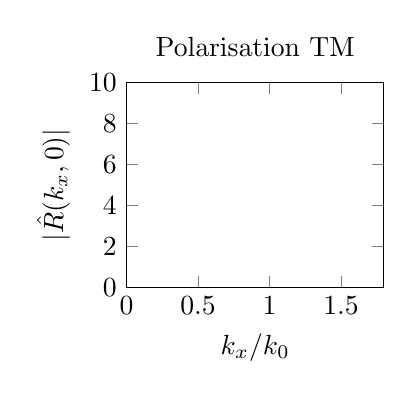
\begin{tikzpicture}[scale=1]
    \begin{axis}[
            title={Polarisation TM},
            ylabel={\(|\hat{R}(k_x,0)|\)},
            xlabel={\(k_x\slash k_0\)},
            width=0.4\textwidth,
            ymin=0,
            ymax=10,
            restrict y to domain=0:+4E+01,
            xmin=0,
            xmax=1.8,
            mark repeat=40,
            legend pos=outer north east
        ]
        % \addplot [color=black,mark=square*] table [col sep=comma, x={s1}, y={Abs(r_ex.tm)}] {csv/SOUDAIS/SOUDAIS.r_ex.MODE_2_TYPE_P.csv};
        % % \addlegendentry{Exact};

        % \addplot [color=blue,mark=x] table [col sep=comma, x={s1}, y={Abs(r_ibc0.tm)}] {csv/SOUDAIS/SOUDAIS.r_ibc.IBC_ibc0_SUC_F_MODE_2_TYPE_P.csv};
        % % \addlegendentry{CI0};

        % \addplot [color=red,mark=diamond*] table [col sep=comma, x={s1}, y={Abs(r_ibc3.tm)}] {csv/SOUDAIS/SOUDAIS.r_ibc.IBC_ibc3_SUC_F_MODE_2_TYPE_P.csv};
        % % \addlegendentry{CI3};
    \end{axis}
\end{tikzpicture}
\tikzsetnextfilename{R_SOUDAIS_plan_hoibc.TE}
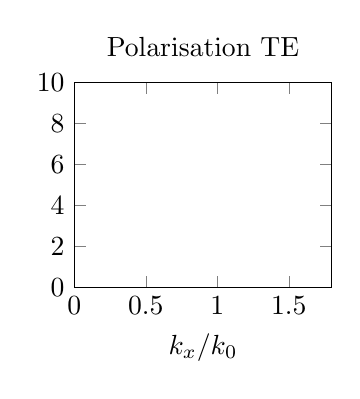
\begin{tikzpicture}[scale=1]
    \begin{axis}[
            title={Polarisation TE},
            ylabel={},
            xlabel={\(k_x\slash k_0\)},
            width=0.4\textwidth,
            xmin=0,
            xmax=1.8,
            ymin=0,
            ymax=10,
            mark repeat=40,
            legend pos=outer north east
        ]
        % \addplot [color=black,mark=square*] table [col sep=comma, x={s1}, y={Abs(r_ex.te)}] {csv/SOUDAIS/SOUDAIS.r_ex.MODE_2_TYPE_P.csv};
        % \addlegendentry{Exact};

        % \addplot [color=blue,mark=x] table [col sep=comma, x={s1}, y={Abs(r_ibc0.te)},color=] {csv/SOUDAIS/SOUDAIS.r_ibc.IBC_ibc0_SUC_F_MODE_2_TYPE_P.csv};
        % \addlegendentry{CI0};

        % \addplot [color=red,mark=diamond*] table [col sep=comma, x={s1}, y={Abs(r_ibc3.te)}] {csv/SOUDAIS/SOUDAIS.r_ibc.IBC_ibc3_SUC_F_MODE_2_TYPE_P.csv};
        % \addlegendentry{CI3};
    \end{axis}
\end{tikzpicture}
      %     \caption[CIOE sur empilement de P.~Soudais p.~11]{Module des coefficients diagonaux de \(\mR\) pour \(\eps = 4, \mu = 1, d=0.035\text{m}, f=12\text{GHz}\)}
      %     \label{fig:reflex_fourier:plan:soudais:hoibc}
      % \end{figure}

      Si la matrice d'impédance exacte possède plusieurs asymptotes, il faut autant de pôles à la CIOE pour être une bonne approximation.

      La figure \ref{fig:imp_fourier:plan:triple_asymptote:hoibc} montre la limite de la CI3 pour capturer 3 asymptotes. Pour cela, il faudrait utiliser une CI d'ordre au moins 6 sur l'opérateur agissant sur \(\vE_t\). La CI3 n'est donc une bonne CIOE que si le nombre d'asymptotes est inférieur à 1, ce que l'on peut calculer connaissant l'empilement (voir proposition \ref{prop:imp_plan:symb_z:1c}).

      L'expression d'une CIOE vérifiant ce critère est la \hyperlink{ci7}{CI7}
      \begin{equation}
        \left(\oI + \sum_{i=1}^3 \left(d_{i} \left(\frac{\LD}{k_0^2}\right)^i + e_{i} \left(-\frac{\LR}{k_0^2}\right)^i \right)\right)\vE_t = \left(a_0 \oI + \sum_{i=1}^3 \left(b_{i} \left(\frac{\LD}{k_0^2}\right)^i + c_{i} \left(-\frac{\LR}{k_0^2}^i\right) \right)\right)\vJ
      \end{equation}

      \begin{figure}[!hbt]
          \centering
          \tikzsetnextfilename{Z_triple_asymptote_plan_hoibc_TM}
\begin{tikzpicture}[scale=1]
    \begin{axis}[
            title={Polarisation TM},
            ylabel={\(\Im(\hat{Z}(k_x,0)\)},
            xlabel={\(k_x\slash k_0\)},
            width=0.4\textwidth,
            xmin=0,
            xmax=1.999,
            ymin=-10,
            ymax=10,
            restrict y to domain=-300:300,
            mark repeat=200,
            legend pos=outer north east
        ]
        \addplot [color=black,mark=square*] table [col sep=comma, x={s1}, y={Im(z_ex.tm)}] {csv/triple_asymptote/triple_asymptote.z_ex.P.csv};
        % \addlegendentry{Exact};

        \addplot [color=blue,mark=x] table [col sep=comma, x={s1}, y={Im(z_ibc0.tm)}] {csv/triple_asymptote/triple_asymptote.z_ibc.IBC_ibc0_TYPE_P_SUC_F.csv};
        % \addlegendentry{CI0};

        \addplot [color=red,mark=diamond*] table [col sep=comma, x={s1}, y={Im(z_ibc3.tm)}] {csv/triple_asymptote/triple_asymptote.z_ibc.IBC_ibc3_TYPE_P_SUC_F.csv};
        % \addlegendentry{CI3};

        \addplot [color=cyan,mark=pentagon*] table [col sep=comma, x={s1}, y={Im(z_ibc7.tm)}] {csv/triple_asymptote/triple_asymptote.z_ibc.IBC_ibc7_TYPE_P_SUC_F.csv};
        % \addlegendentry{CI7};
    \end{axis}
\end{tikzpicture}
\tikzsetnextfilename{Z_triple_asymptote_plan_hoibc_TE}
\begin{tikzpicture}[scale=1]
    \begin{axis}[
            title={Polarisation TE},
            ylabel={},
            xlabel={\(k_x\slash k_0\)},
            width=0.4\textwidth,
            xmin=0,
            xmax=1.999,
            ymin=-10,
            ymax=10,
            restrict y to domain=-300:300,
            mark repeat=200,
            legend pos=outer north east
        ]
        \addplot [color=black,mark=square*] table [col sep=comma, x={s1}, y={Im(z_ex.te)}] {csv/triple_asymptote/triple_asymptote.z_ex.P.csv};
        \addlegendentry{Exact};

        \addplot [color=blue,mark=x] table [col sep=comma, x={s1}, y={Im(z_ibc0.te)}] {csv/triple_asymptote/triple_asymptote.z_ibc.IBC_ibc0_TYPE_P_SUC_F.csv};
        \addlegendentry{CI0};

        \addplot [color=red,mark=diamond*] table [col sep=comma, x={s1}, y={Im(z_ibc3.te)}] {csv/triple_asymptote/triple_asymptote.z_ibc.IBC_ibc3_TYPE_P_SUC_F.csv};
        \addlegendentry{CI3};

        \addplot [color=cyan,mark=pentagon*] table [col sep=comma, x={s1}, y={Im(z_ibc7.te)}] {csv/triple_asymptote/triple_asymptote.z_ibc.IBC_ibc7_TYPE_P_SUC_F.csv};
        \addlegendentry{CI7};                  
    \end{axis}
\end{tikzpicture}
          \caption[CIOE sur empilement avec triple asymptote]{Partie imaginaire des coefficients diagonaux de \(\mZ\) pour \(\eps = 4, \mu = 1, d=0.2\text{m}, f=1\text{GHz}\)}
          \label{fig:imp_fourier:plan:triple_asymptote:hoibc}
      \end{figure}
      \begin{table}[!hbt]
        \centering
        \begin{minipage}[t]{0.49\textwidth}
        \vspace{0pt}
        \centering
        \begin{coefftable}{\hyperlink{ci0}{CI0}}
          \input{csv/triple_asymptote/triple_asymptote.IBC_ibc0_SUC_F_MODE_2_TYPE_P.coeff.txt}
        \end{coefftable}

        \begin{coefftable}{\hyperlink{ci3}{CI3}}
          \input{csv/triple_asymptote/triple_asymptote.IBC_ibc3_SUC_F_MODE_2_TYPE_P.coeff.txt}
        \end{coefftable}
        \end{minipage}
        \tablecoeff[0.49]{\hyperlink{ci7}{CI7}}{csv/triple_asymptote/triple_asymptote.IBC_ibc7_SUC_F_MODE_2_TYPE_P.coeff.txt}
        \caption{Coefficients associés à la figure \ref{fig:imp_fourier:plan:triple_asymptote:hoibc}}
        \label{tab:imp_fourier:plan:triple_asymptote:hoibc}
      \end{table}
